\documentclass[11pt]{article}
\usepackage[toc,page]{appendix}
\RequirePackage{fix-cm}
\usepackage[utf8]{inputenc}
\usepackage[margin=1.5in]{geometry}
\usepackage[bottom, flushmargin]{footmisc}
\setlength{\footnotesep}{\baselineskip} % space between footnotes 
\setlength{\parindent}{0in} % space at start of paragraph
\setlength{\parskip}{0.14in} % space between paragraphs
\linespread{1.25}
\usepackage{titlesec}
\titlespacing\section{0pt}{0.21in}{0.03in}
\titlespacing\subsection{0pt}{0.21in}{0.01in}
\titlespacing\subsubsection{0pt}{0.21in}{0in}
\usepackage{marginnote}
\newcommand{\marnum}[1]{\reversemarginpar \marginnote{#1}[0.14in]}


% bibliography-related packages
\usepackage{natbib}
\setcitestyle{aysep={,}} 
\bibliographystyle{agsm}
\newcommand{\citepos}[1]{\citeauthor{#1}'s (\citeyear{#1})}
\newcommand{\citeshort}[2]{(#1, \citeyear{#2})}

% lists
\usepackage{enumitem} 
\newcommand{\bulletlabel}{\raisebox{0.2ex}{\small$\bullet$}}
\newlist{enumbul}{enumerate}{6}
\setlist[enumbul]{label=\bulletlabel, topsep=0pt, leftmargin=0.3in, rightmargin=0.3in}
\newlist{enumar}{enumerate}{6}
\setlist[enumar]{label=\arabic*$)$,topsep=0pt, leftmargin=0.3in, rightmargin=0.3in}

% packages vital for various things
\usepackage{hyperref}
\usepackage{comment} % commenting out a large chunk
\usepackage{enumitem} % lists
\usepackage{graphicx,nicefrac} % graphics, especially external ones
\graphicspath{ {dataviz/} }
\usepackage{amsmath} % writing math
\usepackage{amssymb} % writing symbols
\usepackage{amsthm}
\usepackage{bm}
\usepackage{float}
\usepackage{mathtools}
\usepackage{bigints}

% colors
\usepackage{tcolorbox}
\usepackage{color} % colors
\usepackage{xcolor, colortbl} % more control over colors
\newcommand{\red}[1]{\color{red}#1\color{black}}
\newcommand{\green}[1]{\color{green!80!black}#1\color{black}}
\newcommand{\blue}[1]{\color{blue}#1\color{black}}
\newcommand{\gray}[1]{\color{gray!80!black}#1\color{black}}
\newcommand{\black}[1]{\color{black}#1\color{black}}

\hypersetup{
	colorlinks,
	linkcolor=black, %internal links
	urlcolor=cyan,  % URLs
	citecolor= black, % references
	breaklinks=true
}

% for use in tables
\usepackage{multirow}
\usepackage{multicol}
\usepackage{array}
\usepackage{booktabs}
\newcommand\bstrut{\rule{0pt}{2.5ex}} % space before row
\newcommand\astrut{\rule[-1.25ex]{0pt}{0pt}} % space after row
\newcolumntype{L}[1]{>{\raggedright\let\newline\\\arraybackslash\hspace{0pt}}m{#1}}
\newcolumntype{C}[1]{>{\centering\let\newline\\\arraybackslash\hspace{0pt}}m{#1}}
\newcolumntype{R}[1]{>{\raggedleft\let\newline\\\arraybackslash\hspace{0pt}}m{#1}}

%miscellaneous
\newcommand{\ansm}[1]{\text{\framebox{\ensuremath{#1}}}}
\newcommand{\anst}[1]{\text{\framebox{#1}}}
\newcommand{\ie}[1][]{\textit{i.e.\ }#1}
\newcommand{\eg}[1][]{\textit{e.g.\ }#1}
\newcommand\pspace {\\[0.07in]}
\newcommand\ppspace {\\[0.14in]}
\newcommand{\logsep}{\begin{center}---------------\end{center}}

\usepackage{tcolorbox}
\def\highlight#1#2{
	\begin{centering}
    
		\vspace{1.2ex}
		\begin{minipage}{0.8\linewidth}
			\begin{tcolorbox}[
				boxsep=3.3pt,
				boxrule=0.4pt,
				colback=white,
				colbacktitle=white,
				coltitle=black,
				colframe=black,
				title=\centering \textbf{#1},
			]
				\centering
				#2
			\end{tcolorbox}
		\end{minipage}
		\vspace{1.2ex}
        
	\end{centering}
}

\begin{document}
\pagenumbering{gobble}

\phantom{Wendy Yu}

\vfill

\begin{center}
\begin{minipage}{0.88\linewidth}
\begin{center}
\LARGE
Centres of Attention: Which Countries are the Most Pivotal in Global Supply Chains? \\[0.21in]
\end{center}
\large This paper develops a novel Pivotal-ness Index to identify and rank countries’ strategic importance in global supply chains across six key dimensions: raw materials, production, consumption, geographic position, digital infrastructure, and future potential. Using computational and econometric methods on granular datasets, I evaluate countries’ roles in supply networks. My findings reveal the complex interdependencies between nations and highlight emerging shifts in supply chain dominance. The results have important implications for understanding geopolitical tensions, economic development patterns, and international trade relationships. This research provides valuable insights for policymakers and businesses in developing strategies to managing critical dependencies.
	\end{minipage}
\end{center}


\vfill

Word Count: 6000 words, including 100-word abstract and 7 figures\\
\phantom{Word Count: 6000 words,} excluding 1 appendix

\newpage
\pagenumbering{arabic}

\section{Motivation}
\label{sec:motivation}

The Bretton Woods conference kicked off an era of globalisation, with countries---almost without exception---becoming more embedded and more reliant on the system of global supply chains which has propelled living standards forward. However, events like the COVID-19 pandemic, Russo-Ukrainian war, and Suez Canal blockage have exposed an underlying fragility to external shocks; supply chains struggled to respond during all 3 events, thus revealing the risk of relying on supply configurations which have no real alternative.

In response, firms and governments have introduced measures to bolster supply chain resilience and protect critical sectors essential for strategic development. Initiatives like the EU Raw Materials Alliance and the US Chips Act aim to secure key industries such as semiconductors, batteries, and pharmaceuticals. Similarly, China’s dual circulation strategy and the Belt and Road Initiative seek to diversify trade routes and mitigate exposure to external shocks.

Accordingly, I am interested in understanding and quantifying the notion of criticality to global supply chains, or what I term as `pivotalness'. It would be highly beneficial to have a robust method of identifying systemic vulnerabilities and dominance structures, with broader implications for policymaking, trade negotiations, and geopolitical stability.

The rest of this paper proceeds as follows. Section \ref{sec:litreview} reviews the relevant literature and situates my research within it. Section \ref{sec:theory} presents the theoretical framework. Section \ref{sec:empirics} outlines the empirical strategy and findings. Section \ref{sec:evaluation} evaluates the robustness of the findings. Section \ref{sec:conclusion} concludes and suggests avenues for future work.

\section{Literature Review}
\label{sec:litreview}

This section focuses on contextualising my notion of `pivotalness'. Relevant frameworks that inform my empirical strategy are discussed in Section \ref{sec:theory}.

Global supply chains arise from the geographic fragmentation of production, allowing countries to specialise according to comparative advantage. Advances in technology foster vertical specialisation \citep{hummels1999} and generate highly interconnected trade networks \citep{baldwin2016}. Electronics supply chains exemplify this phenomenon, with different stages of production dispersed globally. This complexity highlights the need to assess countries’ evolving roles, crucial for securing economic and political stability, strengthening international surveillance, and understanding shifts in global positioning.

Input-output (I-O) analysis is widely used to measure value-added contributions. Studies such as \citet{koopman2014} and \citet{timmer2014} show that high-income economies like the US and Germany embed substantial domestic value in exports, while Asian economies, particularly China, have risen in midstream manufacturing. Research also shows that shocks, such as the 2008 financial crisis \citep{baldwin2009} and China's COVID-19 lockdown \citep{lafrogne2022}, produce ripple effects across supply chains, highlighting vulnerabilities at both upstream and downstream stages. However, traditional I-O studies often use aggregated data, limiting granularity. My research complements these approaches by using more detailed trade data to examine niche critical suppliers.

Parallel research using trade network analysis examines structural positions of countries. Analyses by \citet{de2014network} and \citet{deguchi2014hubs} identify central nodes within trade networks. \citet{cingolani2017} shows how upstream, midstream, and downstream roles differ across countries, while \citet{alves2022} highlights how shifts in technological capacity, market forces, and policy reshape these roles over time. My essay builds on these frameworks, using extensive data to map changes in country pivotalness across production stages.

Despite the rich literature, many studies focus on short timeframes, specific industries, or isolated countries. Research on geographic, digital, and financial participation exists but tends to address these dimensions separately. This essay bridges that gap by integrating tangible (physical goods) and intangible (financial and digital) networks into a unified pivotalness framework. Moreover, much of the existing work predates the pandemic and the current escalation of geopolitical tensions. Thus, my contribution provides an updated, holistic framework to assess countries’ pivotal roles in global supply chains, capturing how complex interdependencies shape international dominance.


\section{Theoretical Framework}
\label{sec:theory}

In general, I define \textbf{pivotal} in the following context: A country that is deemed \textbf{pivotal} is the one that plays a central role in ensuring the smooth functioning, efficiency, and resilience of the entire supply chain, where its role has short-term irreplaceability. 

\highlight{Pivotal Type 1: Raw Materials}{If this country does not extract raw materials, there will be a significant impact on the industries that use those raw materials.}

The extraction of raw materials is the initial stage of the supply chain and the inputs for later production. Instead of looking at plant-based or animal-based raw materials, this essay will focus on mining-based materials (e.g., iron ore, cobalt, and fossil fuels) that are used for industrial inputs and are of greater economic significance compared to the other two categories. In particular, the government has been increasingly concerned about critical raw materials (CRM). They are materials used in sectors with high economic (e.g., technology) or strategic importance (e.g., national defence, space and technology) and are exposed or will be exposed to high supply risks \citep{european2023}. The CRM lists vary among countries due to differences in development and industrial structure. However, lists from major trading nations show that there are many overlaps. This could be attributed to the green energy transitions and escalating geopolitical tensions, where policymakers started prioritising the security of CRM supply to guarantee a sustainable supply chain \citep{kowalski2023}.
 
CRMs are classified with complicated and differential methods based on different contexts of countries, but common aspects include material scarcity, economic and geopolitical importance, supply or production risks, substitutability, geographic concentration, etc \citep{mancini2016}. However, the pivotalness concept did not intend to capture material scarcity as part of the criticality measure, as industrial changes may reduce a CRM’s criticality in the longer run. Despite this, many materials used in the renewable energy sector will remain important in the future due to the industry's essentiality \citep{kowalski2023}. Therefore, countries that were major exporters of these CRM are clearly pivotal to the supply chain.  

\highlight{Pivotal Type 2: Production}{If this country does not perform its manufacturing function, there will be a significant impact both upstream and downstream.}

Given the rise in geopolitical tensions and the US-China trade war, supply chain reconfiguration is underway, with moves toward friend-shoring, back-shoring, and near-shoring. However, this indirectly reinforced the presence of manufacturing hubs like China, which remain dominant and only partially substitutable, due to complex supply chain interdependencies \citep{alfaro2023}. In the short run, shifting away from existing hubs is challenging and involves a great efficiency trade-off for major importing countries, which tackles our concept of ‘pivotalness’. Studies from \citet{scheibe2018} directly apply to intermediate manufacturing as well as the pivotal types 1 and 3 — any disruption at any stage could propagate throughout the entire supply chain due to feedback loops, tight coupling, and interdependencies. This is supported by the recent COVID-19 lockdowns in Chinese factories \citep{lafrogne2022}.

The interdependencies of the supply chain require an examination of intermediate goods, which are inputs used in the production of final goods and services. In general, developing nations tend to take a larger share of intermediate goods exports due to primarily lower labour costs \citep{lazard2023supplychains}, while developed nations skew less. In order to study the pivotalness of different countries from this ‘input good’ perspective, a theoretical approach which accounts for the aforementioned supply chain interdependencies is required. The best current method for doing so is via the use of input-output tables \citep{leontief1951}, which allow us to trace the entire global supply chain leading to the purchase of a final good or service. Given its proven record of robustness in studying supply chains, it is a good theoretical choice to underpin my empirical strategy.

\highlight{Pivotal Type 3: Consumption}{A country is a pivotal consumer if - upon closing its markets to international trade - there will be a significant reduction in the final demand felt by other countries.}

The framework here is very similar to Pivotal Type 2 (production), except that it examines final demand at the end of the supply chain, rather than intermediate supply. It is important to study consumption pivotalness because major shifts in consumer demand have historically had major supply chain ramifications \citep{fernandez2019}, such as during the COVID-19 recession and the 2008 financial crisis, where contractions in final demand were amplified throughout the entire supply chain \citep{baldwin2009}. This is also known as the bullwhip effect \citep{lee1997}. Even though supply chains were able to recover after the events, the short-term inefficiencies and disruptions were non-negligible. Furthermore, these shocks often incentivise firms to shift sourcing strategies, eventually altering trade flow and patterns in the longer run \citep{ferrari2025}.
 
Similar to pivotal type 2, input-output tables are the most theoretically robust way to capture these interlinkages; for parsimony, I will not repeat the justification.


\highlight{Pivotal Type 4: Geographic}{If something goes wrong in this country, physical trade pathways will be heavily affected.}

Trade heavily depends on physical logistics to ensure the efficiency in transporting raw materials, intermediate goods and final products across countries. According to \citet{unctad2023}, over 80\% of traded goods by volume to transported via seaborne trade. Therefore, Pivotal Type 4 must study the notion of ‘connections’, defined as a country’s integration into and accessibility within the global trade logistics networks by sea, air, and land. This notion is theoretically underpinned by transport geography \citep{rodrigue2012,hesse2020} and the Global Production Networks (GPN) framework (Coe and Yeung, 2015), which emphasise that well-connected logistic hubs serve as critical nodes that enable the smooth flow of trade. Connections are not only crucial for the physical flow of goods but also for overall supply chain resilience. Empirical research shows that countries with strong logistical linkages are more capable of responding to shocks, rerouting flow and maintaining supply chain continuity (Baldwin et al., 2023). 

Recent events such as the Suez Canal blockage (2021), the Red Sea crisis (2024), and the Baltimore Bridge Collapse (2024) highlight the presence of logistical chokepoints, maritime routes and critical infrastructure, where their disruption causes delays and drops in global trade volume \citep{unctad2024}. Overall, disruptions in pivotal logistical hubs would lead to widespread inefficiencies across the entire supply chain, given their short-term irreplaceability and vulnerabilities to external shocks \citep{baldwin2023}.

\highlight{Pivotal Type 5: Digital}{If something goes wrong with this country’s digital infrastructure, global online activity will be significantly impacted.}

Today, modern supply chains are largely incorporating digital technologies (e.g., AI, IoT, and blockchain) to improve efficiency and adaptability by operating functions such as demand forecasting and logistics streamlining. Although digitalisation in supply chains is driven primarily by technological advancements, it has become increasingly important in recent, volatile economic contexts. Firms are increasingly reliant on digital platforms to operate their supply chains, as they enable quick responses, such as re-routing trucking and shipping during chokepoint closures, to disruptions or changes in market conditions. Given the importance of digital technologies, it suggests the criticality of their underlying infrastructure. 
 
Given the nature of infrastructure, they have high barriers to entry (e.g., complex technologies and construction time), making them hardly substitutable in the short run \citep{jurgens2025}. Therefore, they are strong and tangible proxies to exhibit a country’s digital capacity and infrastructural role underlying digital pivotalness. 

Meanwhile, the reliance on digital networks and flow has exposed global supply chains to new vulnerabilities, such as cybersecurity risks and sabotage of physical infrastructures (e.g., the 2022 Submarine Cable attacks). Likewise, governments could weaponise these data centres to achieve political objectives \citep{farrell2019}, which may incur great inefficiencies in the operating digital networks. . 

\highlight{Pivotal Type 6: Financial}{A country is financially pivotal if a disruption to its financial infrastructure would significantly impair the functioning of global trade and supply chains.}

Financial infrastructure (e.g., clearing systems, payment systems and banks) acts as a backbone for efficient and smooth trade. It plays a crucial role in mitigating risks, enhancing liquidity between suppliers and buyers, and, thereby, facilitating and enabling cross-border trade (ICC, 2013). Previous financial crises, notably the 2008-09 financial crisis, indicate that disruptions and collapse of major financial hubs (e.g., the US, UK) significantly undermine trade flows (BIS, 2014). The ongoing geopolitical tensions such as trade wars and sanctions imposed by major trading nations, would largely increase cost of financing and related currency risks \citep{bednarski2023}. These events can disrupt the smooth operation of supply chains, hence revealing vulnerabilities underpinning our concept of pivotalness.

In theory, the concept of financial pivotalness would ideally be measured through a combination of indicators that capture a country's embeddedness in the global financial system. These might include the country's share of global cross-border payment traffic and the total value of transactions processed by domestic clearing and settlement systems that support international trades. These measures often provide a multidimensional view of how central a country is to the financial infrastructure that supports global supply chains, and how sensitive international trade would be to financial disruptions originating from that jurisdiction.


\section{Empirical Strategy \& Findings}
\label{sec:empirics}

This section details the computational and econometric methods to evaluate countries’ pivotal roles across six dimensions of global supply chains. The approach comprises two layers: (1) computational analysis to derive subindices for each pivotal type using diverse, granular datasets, and (2) econometric analysis to synthesise these into a unified Pivotal-ness Index and project future trends. Each pivotal type’s data sources, processing steps, and analytical framework are elaborated below, reflecting the current date of March 1 2025, for data timeliness.

\subsection{Raw Materials}

For raw materials pivotalness, I use trade data from the CEPII BACI database \citep{baci2023}, covering the period from 1995 to 2023. The analysis focuses on a curated list of critical raw materials\footnote{The raw materials covered include iron ores, rare earth elements, cobalt ores, lithium, critical fertilisers, and other commodities essential for industrial production and supply chain stability. The codebase contains complete list of HS codes used in \texttt{dep/hs\_list.py}.}. Only cross-border exports of primary raw materials are considered, excluding downstream manufactured goods, to ensure the analysis targets upstream vulnerabilities rather than processing or value-added trade.

For each country, I aggregate the value of exported critical raw materials and compute its share of global raw material exports. Each country’s pivotalness score is then normalised to an index where 100 represents the country most critical to global raw material supply in each year. Figure \ref{fig:pivotal_raw} presents a snapshot of the results for 2023, showing the top 20 countries by raw material pivotalness.

\begin{figure}[H]
	\caption{Raw Materials Pivotalness: 1999–2023}
	\label{fig:pivotal_raw}
	\centering
        \phantom{a}
	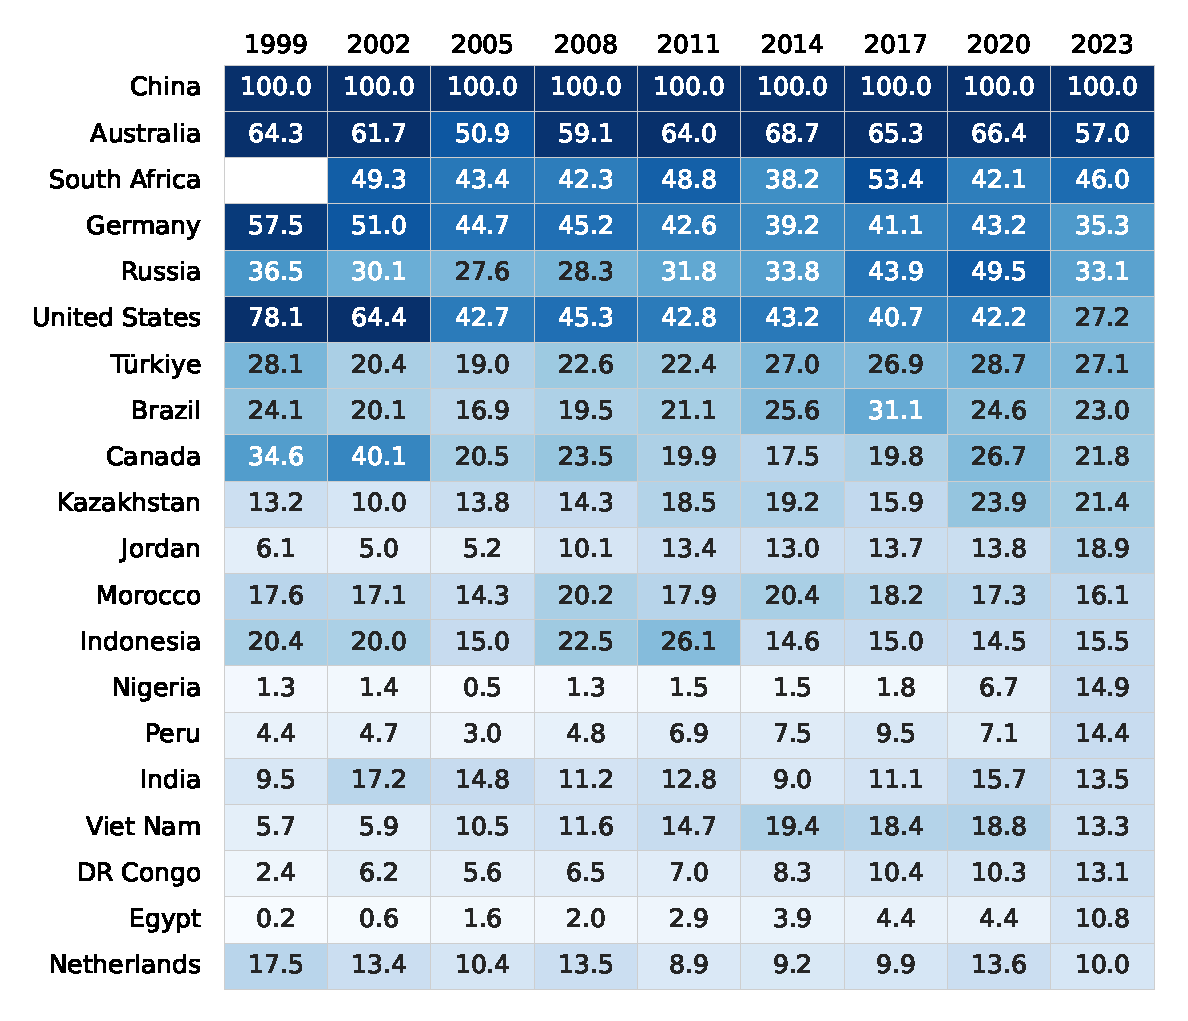
\includegraphics[width=\textwidth]{dataviz/results_pivotal1_snapshot.eps}

	{\footnotesize Source: Author's calculations based on CEPII BACI data.}
\end{figure}

The results highlight China's dominant role in the global raw materials supply chain, holding the maximum possible value for CRM pivotalness across the entire period. This reflects China’s centrality in supplying a broad range of critical inputs—particularly rare earths, graphite, tungsten, and speciality minerals used in electronics, defence, and renewable energy technologies.

Australia emerges as the second-most pivotal country, with a score of 19.5 in 2023. Australia's pivotalness is primarily driven by its dominant exports of iron ore, lithium, and critical mineral concentrates, all crucial for both industrial manufacturing and the global energy transition. South Africa ranks third, anchored by its leadership in platinum group metals (PGMs), vanadium, and chromium supply chains, despite fluctuations in its annual pivotalness. Germany and Russia also feature among the top suppliers, reflecting their specialised roles in industrial minerals and energy-related commodities, although both have shown gradual declines in pivotalness over the past two decades. By contrast, the United States has seen a sharper decline—from a pivotalness score of 27.7 in 1999 to just 9.3 in 2023—reflecting its relative withdrawal from primary resource exports amid growing import reliance.

Overall, the findings illustrate that raw material pivotalness remains highly concentrated, with a handful of countries playing disproportionately large roles in enabling global manufacturing and technological ecosystems. Given rising geopolitical tensions and the accelerating demand for critical minerals, monitoring shifts in raw materials pivotalness will be essential for understanding future vulnerabilities in global supply chains.


\subsection{Production}

For production pivotalness, I use data from the OECD Inter-Country Input-Output (ICIO) Tables \citep{oecdicio2023}, covering the period from 1995 to 2020. The analysis focuses on the export of intermediate goods, excluding final demand sectors such as household consumption and gross fixed capital formation\footnote{Specifically, sectors associated with final demand—HFCE, GFCF, INVNT, and similar categories—are excluded to isolate purely intermediate trade flows.}. Only cross-border transactions are considered, ensuring that domestic flows do not distort the identification of global midstream hubs.

For each country, I sum the value-added embedded in exported intermediate goods and services, expressed in USD millions. Each country's share of global intermediate exports is then normalised to an index where 100 represents the most pivotal production economy in each year. Figure \ref{fig:pivotal_production} presents a snapshot of the results for 2020, showing the top 20 production hubs by pivotalness.

\begin{figure}[ht]
	\caption{Production Pivotalness: 1999–2020}
	\label{fig:pivotal_production}
	\centering
        \phantom{a}
	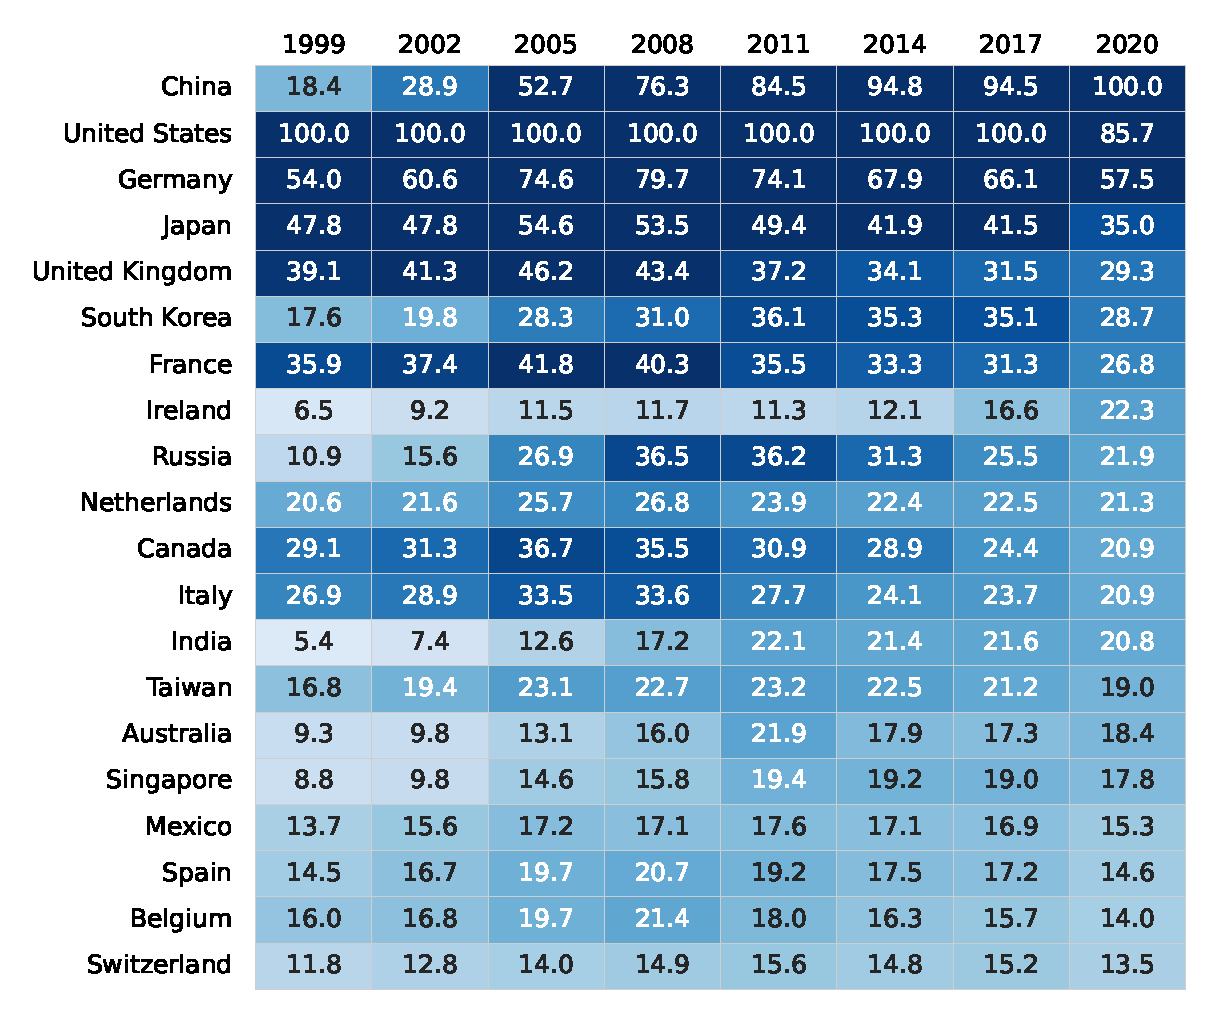
\includegraphics[width=\textwidth]{dataviz/results_pivotal2_snapshot.eps}

	{\footnotesize Source: Author's calculations based on OECD ICIO Tables.}
\end{figure}

The results reveal the overwhelming dominance of China as a midstream production hub. In 2020, China scores the maximum pivotalness value of 100.0, reflecting its extraordinary role in supplying intermediate goods to global supply chains. Germany (57.5), the United States (41.2), and Japan (35.0) follow at a significant distance. China's position stems from its concentration in key sectors such as electronics (semiconductors, circuit boards), machinery components, textiles, and light industrial manufacturing, confirming its status as the world's most entrenched midstream economy.

Germany ranks second with a diversified industrial base spanning automotive parts, advanced machinery, and chemical intermediates. Although its relative pivotalness has declined slightly over the period, Germany remains a critical supplier to European and global manufacturing networks. The United States maintains high pivotalness through sectors such as aerospace, high-technology machinery, and advanced electronics, although its share of broader intermediate manufacturing exports has steadily eroded over time. Emerging economies, notably Vietnam and Mexico, show upward trends in pivotalness, supported by global diversification efforts such as friendshoring and nearshoring. However, their absolute pivotalness scores remain modest compared to the entrenched dominance of China and Germany. Taiwan ROC, despite its relatively small size, features strongly due to its outsized role in semiconductor fabrication—a sector whose strategic importance has become increasingly evident post-pandemic.

An important dynamic observable across the panel is the "stickiness" of production pivotalness. Despite rising wages in China and efforts to reconfigure supply chains, inertia, industrial clustering, and cumulative investment advantages have entrenched China’s centrality. Temporary shocks, such as factory shutdowns in Vietnam during 2021, reveal how even secondary hubs have become essential to global stability. Nevertheless, meaningful reconfiguration is underway, with gradual shifts toward regional diversification. Yet in the medium term, global intermediate manufacturing pivotalness remains highly concentrated in a few economies, and remains difficult to rapidly substitute.

\subsection{Consumption (Final Demand)}

For demand pivotalness, I use data from the OECD Inter-Country Input-Output (ICIO) Tables \citep{oecdicio2023}, covering the period from 1995 to 2020. To capture each country’s role as a driver of global final demand, I extract cross-border flows associated with final consumption and investment sectors.\footnote{Specifically: Household Final Consumption Expenditure (HFCE), Non-Profit Institutions Serving Households (NPISH), Government Final Consumption (GGFC), Gross Fixed Capital Formation (GFCF), changes in inventories (INVNT), and direct purchases abroad by residents (DPABR).} Only imported final goods and services are considered, excluding domestic absorption and intermediate inputs, to ensure the analysis focuses on external demand pressures.

The metric measures, for each country, the total value of imported final demand, expressed in USD millions. Each country’s share of global imported final demand is then computed and normalised to an index where 100 represents the most pivotal market in each year. Figure \ref{fig:pivotal_demand} presents a snapshot of the results for 2020, showing the top 20 markets by demand pivotalness.

\begin{figure}[H]
	\caption{Demand Pivotalness: 1999–2020}
	\label{fig:pivotal_demand}
	\centering
        \phantom{a}
	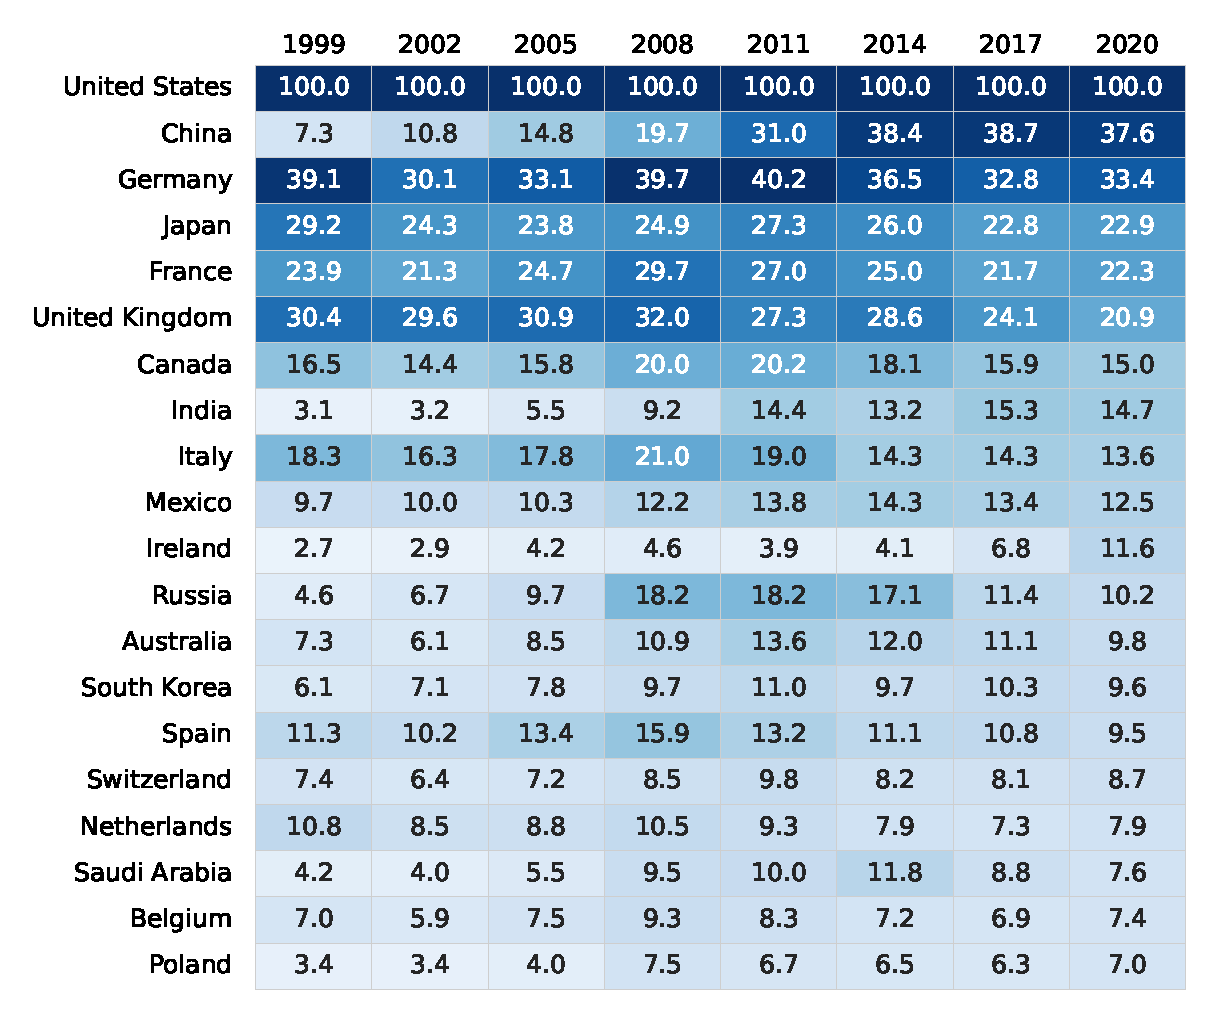
\includegraphics[width=\textwidth]{dataviz/results_pivotal3_snapshot.eps}

	{\footnotesize Source: Author's calculations based on OECD ICIO Tables.}
\end{figure}


The results confirm that the United States remains the world's most important source of final demand across the entire period. The scale of US demand is particularly evident in 2020, when it accounted for nearly 20\% of global imported final goods. However, the analysis also highlights evolving dynamics: China has now surpassed Germany to become the second-most pivotal market, achieving a score of 37.6 compared to Germany’s 33.4. This reflects China’s gradual shift towards greater domestic consumption and investment, complementing its role as a global manufacturing hub.

Japan, France, and the United Kingdom form a closely grouped second tier, each maintaining significant, though declining, influence over global demand patterns. Canada, India, and Italy also remain important, with India showing modest but consistent gains over time. Notably, despite long-standing slow growth, Japan’s resilience in pivotalness underscores the inertia embedded within mature consumption and investment systems.

Overall, while global demand pivotalness remains highly concentrated among a few large economies, gradual eastward shifts are visible, particularly driven by China and, to a lesser extent, India. Nevertheless, the structural gap between the United States and all other economies remains wide, reinforcing the outsized influence of US demand on the configuration and stability of global supply chains.

\subsection{Geographic}

For geographic pivotalness, I compile data from three complementary sources: the United Nations Conference on Trade and Development’s Liner Shipping Connectivity Index (LSCI) for maritime shipping \citep{unctad2023lsci}, the World Bank’s Logistics Performance Index (LPI) for air transport connectivity \citep{worldbank2023lpi}, and a dataset of international land borders from the World Population Review \citep{wpr2025landborders}. To reflect the true distribution of global trade flows across these channels, I apply weighted averaging: maritime connectivity is assigned a weight of 80\%, air connectivity 18\%, and land connectivity 2\%. These weights are based on UNCTAD estimates indicating that approximately 80\% of global trade by volume is transported by sea, with air and land accounting for much smaller shares \citep{unctad2023}\footnote{Although air freight accounts for a larger share of global trade \textit{by value}, its volume share remains low, typically below 2\%.}. This weighting ensures that the index appropriately emphasises the modes of transport that dominate physical trade movements. The final pivotalness score thus captures a country’s systemic importance in enabling the efficient global flow of goods across sea, air, and land routes. Figure \ref{fig:pivotal_geographic} presents a summary of the results, for the top 20 countries only:

\begin{figure}[H]
	\caption{Geographic Pivotalness: 2006–2023}
	\label{fig:pivotal_geographic}
	\centering
        \phantom{a}
	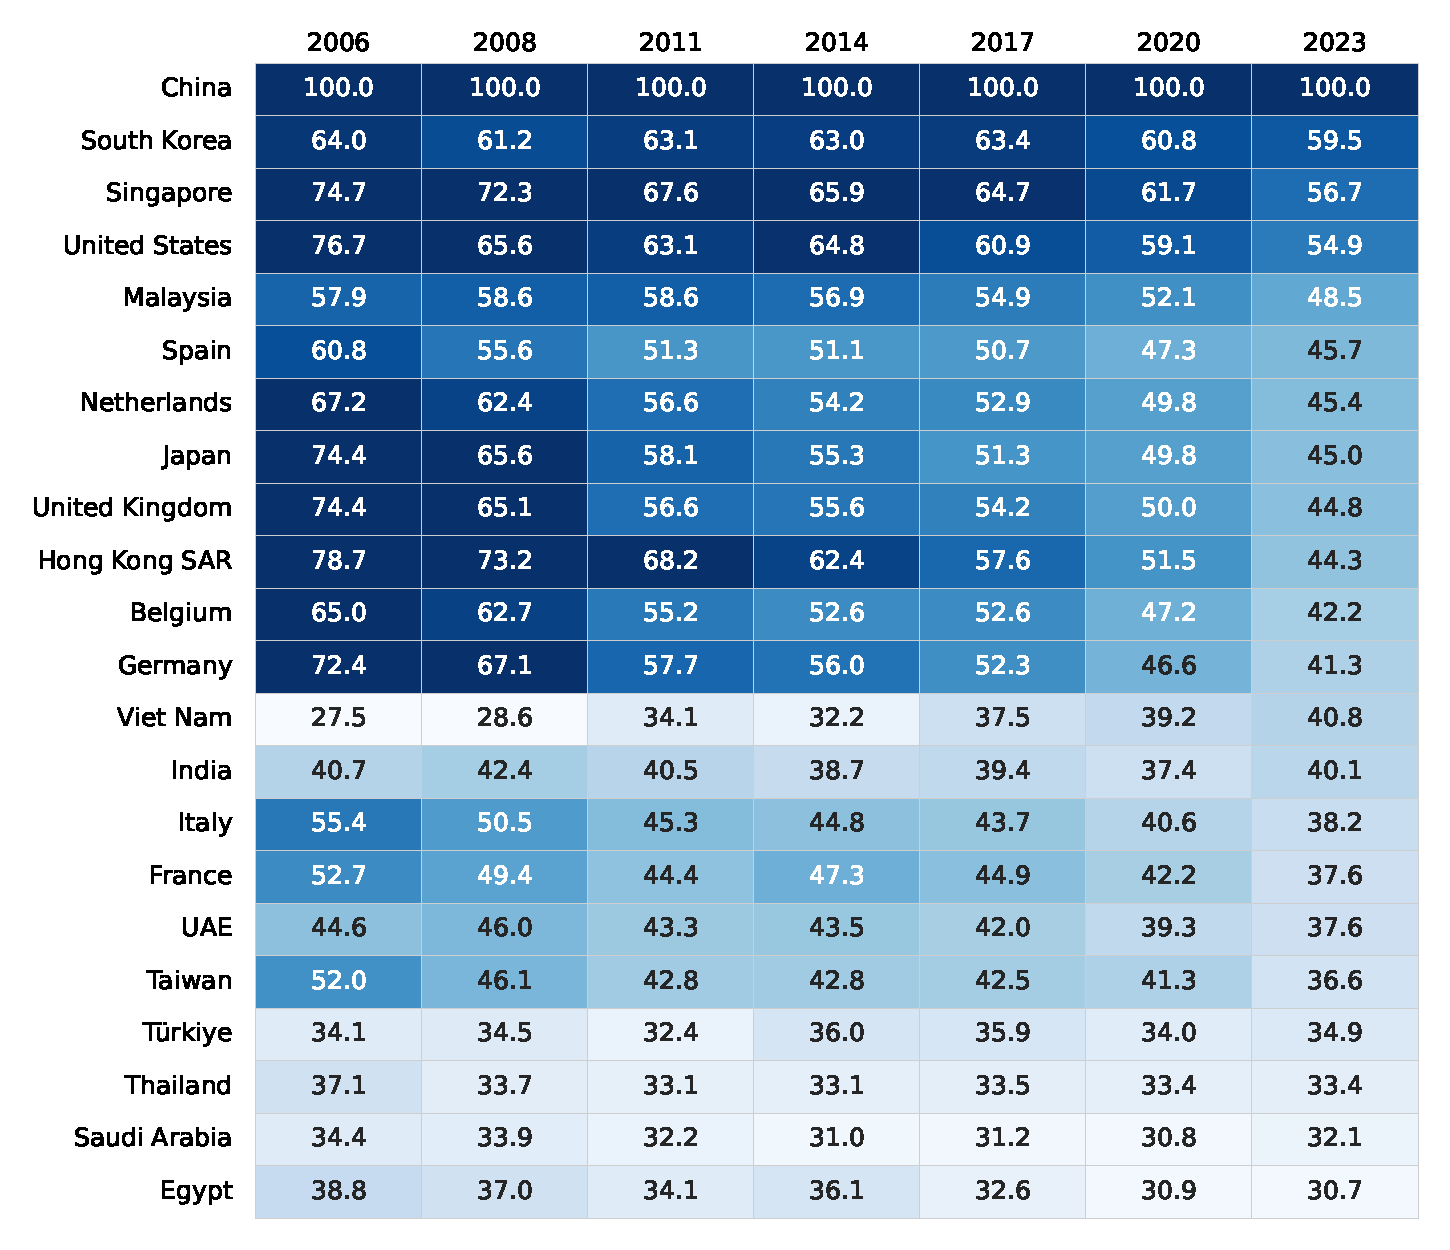
\includegraphics[width=\textwidth]{dataviz/results_pivotal4_snapshot.eps}

	{\footnotesize Source: Author's calculations based on data from UNCTAD LSCI, World Bank LPI, and World Population Review.}
\end{figure}

The data reveals the exceptional and consistent dominance of China in global geographic pivotalness. Across all surveyed years from 2006 to 2023, China maintains a perfect index value of 100, underscoring its irreplaceable role in global trade infrastructure, both maritime and overland. This durability reflects not only China’s manufacturing centrality but also its sustained investments in port expansions, airport hubs, and cross-border logistics corridors such as the Belt and Road Initiative. Other Asian economies—most notably South Korea and Singapore—rank immediately behind China, although both have experienced gradual erosion in relative pivotalness over time. Singapore’s decline from 74.7 to 56.7 reflects both the rise of regional competitors and the physical constraints faced by a city-state. Nevertheless, it remains a critical maritime and air transshipment point, a role shared by Malaysia, which notably punches above its economic weight from a GDP share perspective.

The United States, while maintaining a high early position, exhibits a steady downward trajectory, dropping from 76.7 in 2006 to 54.9 by 2023. This trend mirrors broader shifts in global trade gravity towards Asia. Although the US continues to command vast air and land connectivity, it faces increasing competition from emerging Asian hubs and a declining share of global maritime traffic. Europe’s traditional powers—Germany, Belgium, France, and the Netherlands—also display slow but persistent decline. While these countries remain vital regional logistics nodes, their global centrality has diminished, a trend amplified by infrastructure limitations and the consolidation of trade flows through larger, newer mega-hubs elsewhere.

Among emerging economies, Vietnam stands out as a remarkable climber, rising from a pivotalness score of 27.5 in 2006 to 40.8 in 2023. This surge reflects Vietnam’s growing role as an alternative manufacturing and export base, particularly in the aftermath of US–China trade tensions. India also shows steady progress, though from a higher base, driven by investments in port capacity, airport modernisation, and logistics corridors.

Overall, the findings portray a geographic landscape undergoing a slow but undeniable eastward shift. While traditional players remain important, the gravitational centre of global logistics is increasingly anchored in Asia, with new hubs steadily ascending alongside the old. Geographic pivotalness proves relatively sticky—rarely gained or lost quickly—but long-term infrastructure investment and global trade realignment are visibly reshaping the hierarchy of global transport connectivity.


\subsection{Digital}

For digital pivotalness, I use data from the Data Center Map \citep{datacentermap2023} and Submarine Cable Map \citep{submarinecablemap2023}, which are comprehensive sources of data on global data centres and submarine cable infrastructure, respectively. These two components jointly capture the physical infrastructure that underpins the global internet and data economy. Submarine cables are the backbone of international connectivity, carrying over 95\% of intercontinental internet traffic \citep{noaa2024}, while data centres function as the primary nodes for storing, processing, and routing digital information.

To construct a digital pivotalness index, I compile the total number of active submarine cable landings and commercial data centres for each country as of 2023. Due to the prohibitive cost of acquiring full time series data, I am only able to produce a snapshot for 2023. Each metric is normalised relative to the maximum observed value across all countries, yielding two sub-indices ranging from 0 to 100. I then compute the unweighted average of these two sub-indices to form the overall digital pivotalness score. This  offers a clear, interpretable measure of a country’s structural importance to the digital layer of global supply chains. Figure \ref{fig:pivotal_digital} presents a summary of the results, for the top 20 countries only:

\begin{figure}[H]
	\caption{Digital Pivotalness: 2023}
	\label{fig:pivotal_digital}
	\centering
        \phantom{a}
	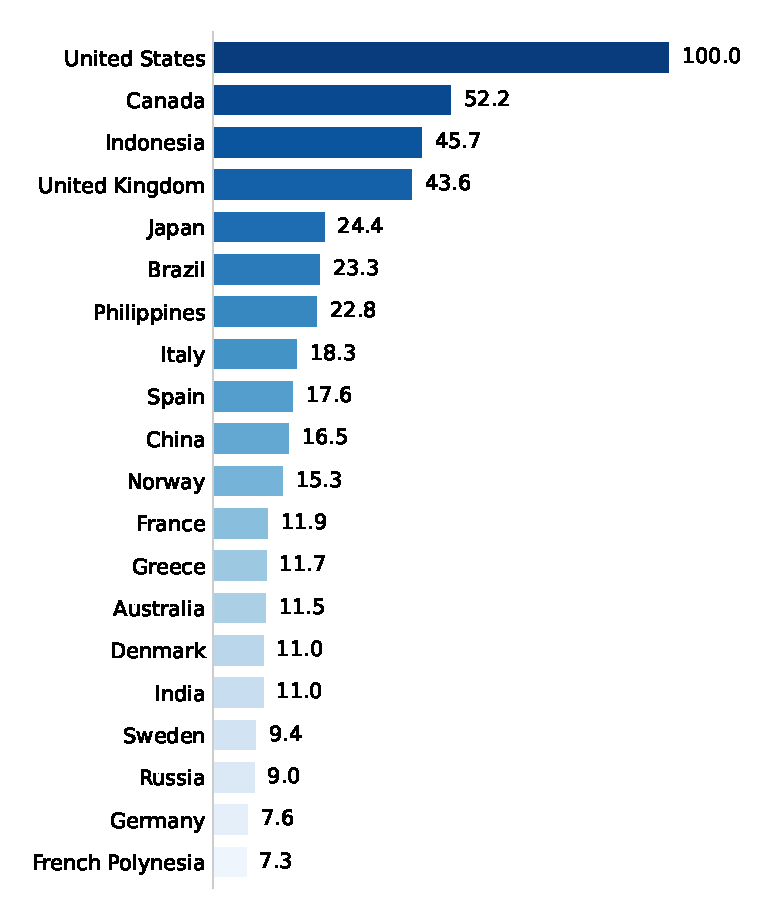
\includegraphics[width=0.7\textwidth]{dataviz/results_pivotal5_snapshot.eps}

	{\footnotesize Source: Author's calculations based on data manually compiled from maps provided by the \citet{datacentermap2023} and \citet{submarinecablemap2023}.}
\end{figure}

The results, shown in Figure \ref{fig:pivotal_digital}, reveal the exceptional dominance of the United States in global digital infrastructure, with a digital pivotalness score of 100.0. This reflects the country's unparalleled number of both submarine cable landings and commercial data centres. The next closest countries — Canada (52.2), Indonesia (45.7), and the United Kingdom (43.6) — register less than half the US score, highlighting the asymmetry in global digital intermediation.

Interestingly, several emerging economies appear in the top 10, including Indonesia, the Philippines, and Brazil. Their presence reflects a growing role as regional digital hubs, likely driven by population size, increasing digital demand, and recent infrastructure investments. In contrast, traditional digital powers such as Germany (7.6), Sweden (9.4), and France (11.9) rank relatively lower, suggesting that submarine cable landings — concentrated in maritime-accessible or island nations — may skew the metric in favour of coastal and archipelagic states.

China, despite its advanced digital ecosystem, ranks only 12th with a score of 16.5, likely due to the limited number of foreign-operated data centres and fewer international submarine cable landings compared to Western peers. Overall, the index reveals a highly concentrated digital core, where a handful of countries play outsized roles in enabling the infrastructure behind global data flows.

\subsection{Financial}

For financial pivotalness, I use data from the Bank for International Settlements (BIS) Triennial Central Bank Survey, specifically focusing on foreign exchange (FX) turnover (covering spot transactions, outright forwards, foreign exchange swaps, currency swaps, and FX options) as a measure of financial pivotalness. Using FX turnover data from the BIS Triennial Survey to measure financial pivotalness is justified on three grounds. First, high FX turnover signals a country’s central role in global trade and capital flows, with key hubs like the USA, UK, Singapore, and Hong Kong acting as major intermediaries. Second, the ability to process large volumes of FX transactions reflects strong financial infrastructure—deep banking systems, stable regulations, and legal frameworks—all crucial for global intermediation. Third, the BIS survey adjusts for local and cross-border double-counting, making it a robust and credible source for cross-country analysis.

After compiling the data from BIS Triennial Surveys from 1995 to 2022, I convert it into an indexed form, with 100 representing the most financially pivotal jurisdiction in each survey year. \ref{fig:pivotal_financial} presents a summary of the results, for countries with an index greater than 1 only:

\begin{figure}[H]
	\caption{Financial Pivotalness: 1995 to 2022}
	\label{fig:pivotal_financial}
	\centering
        \phantom{a}
	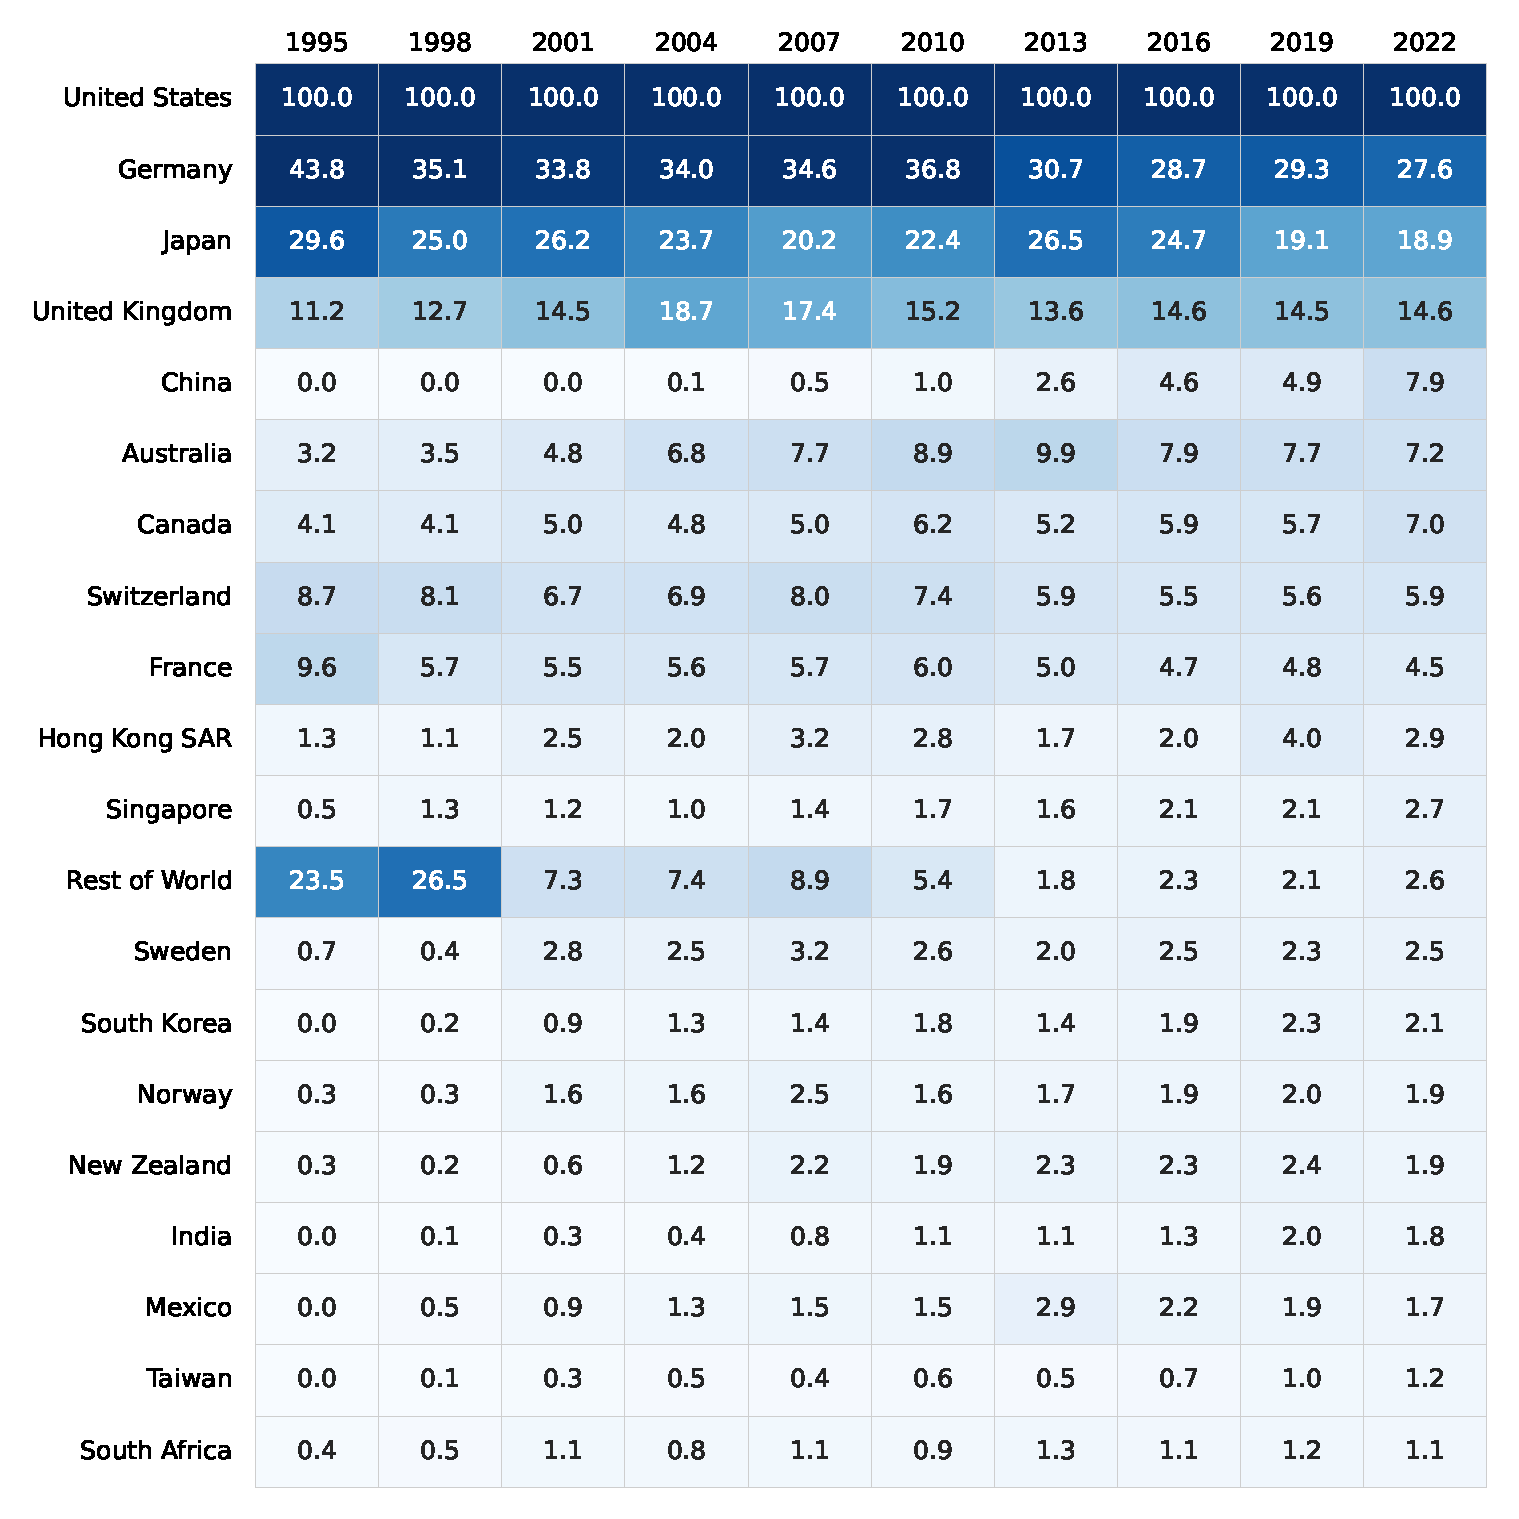
\includegraphics[width=\textwidth]{dataviz/results_pivotal6_snapshot.eps}
	{\footnotesize Source: Author's calculations based on BIS Triennial Surveys.}
\end{figure}

The data reveals the uninterrupted dominance of the United States in global financial intermediation. Across all survey years from 1995 to 2022, the US holds a value of 100, making it the anchor point for comparison and underscoring its exceptional and persistent centrality in global FX markets. This reflects the structural role of the US dollar in international trade, financial contracts, and reserve holdings.

Germany and Japan emerge as the second and third-most pivotal countries over the long run, with average index values of 33.4 and 23.6, respectively. While both countries show modest declines over the decades, their continued presence in the upper tier of the distribution speaks to their long-standing integration into global capital markets. The United Kingdom shows a steady trajectory, averaging 14.7, consistent with London’s role as a leading FX trading hub despite geopolitical and regulatory shifts, including Brexit. Notably, a handful of mid-ranked financial centres such as Switzerland (6.9), Australia (6.8), France (5.7), and Canada (5.3) display relatively stable scores over time, suggesting they function as regional or specialised financial nodes in the broader FX network.

At the lower end of the scale, several emerging economies, including China, have risen from near-zero levels in the 1990s to more measurable levels in recent years. China’s relative index value reached 7.9 in 2022, reflecting the gradual internationalisation of the renminbi and its increased participation in cross-border financial flows. Nonetheless, its long-run average (2.2) remains modest, reinforcing the notion that currency convertibility and institutional openness remain barriers to financial centrality. It should be noted that the decline of the ‘Rest of World’ category from 23.5 in 1995 to just 2.6 in 2022 is primarily due to the creation of the Euro in 1999. Nevertheless, this further highlights the concentration of financial pivotalness in a shrinking set of core jurisdictions. Overall, this sub-index paints a picture of a highly asymmetric financial system, where a small number of countries play an outsized role in enabling global trade, investment, and liquidity flows.

\subsection{Overall Index: Principal Component Analysis}

\subsection{Potential for Forecasting}

\section{Discussion} 
\label{sec:evaluation}

For each pivotal type, I pose a key question: In what way might the numbers I have found not fully capture the conceptual definition of pivotalness, namely short-term irreplaceability with significant global impact? This evaluation highlights potential misalignments while offering context to defend the robustness of the results.

For \textbf{critical raw materials}, the metric could overemphasise trade visibility rather than true production control. A country may appear pivotal by re-exporting resources extracted elsewhere, as seen with South Africa’s role in the diamond trade. However, this risk is mitigated by my deliberate selection of upstream HS codes, ensuring focus on genuine extraction points. Furthermore, intermediary hubs themselves often represent critical chokepoints in early-stage resource flows.

For \textbf{production pivotalness}, value-added export figures might reflect economic scale more than specialised irreplaceability. Germany, the US, and China dominate due to industrial breadth, while Taiwan’s dominance in semiconductors shows that niche supremacy can matter more than size. Nevertheless, scale itself confers resilience: highly embedded economies are harder to substitute, and specialisation is still visible among top-ranked countries.

For \textbf{demand pivotalness}, final goods import shares could simply mirror market size rather than true supply chain centrality. Yet even flexible large economies, such as the US, exert outsized gravitational pull: as demonstrated during the 2025 'reciprocal tariff' episode, shifts in US demand quickly reconfigure global production, pricing, and logistics. Thus, size and systemic pivotalness are fundamentally intertwined.

For \textbf{geographic pivotalness}, reliance on trade through chokepoints could exaggerate irreplaceability if rerouting options exist. However, even when alternatives like the Cape of Good Hope exist, supply chains experience serious delays, cost increases, and insurance risks. Furthermore, not all chokepoints are equally substitutable, and the metric captures the critical friction introduced by disruption, not absolute immobility.

For \textbf{digital pivotalness}, submarine cable landings and data centre numbers could be seen as indicators of volume rather than vulnerability. Yet physical realities — submarine bottlenecks like Singapore, Djibouti, Marseille — mean that certain nodes remain critical. Cable cuts, cyberattacks, or regulatory shutdowns at these points have historically caused severe slowdowns. Thus, digital pivotalness appropriately reflects enduring infrastructure vulnerabilities beneath virtual networks.

For \textbf{financial pivotalness}, BIS FX turnover data includes more than trade finance, potentially overstating financial intermediation. However, supply chains are deeply financialised, relying on robust FX markets for payments, risk management, and earnings repatriation. FX turnover also offers rare, globally standardised, geographically disaggregated data. Hence, while broader than trade flows alone, the measure remains a powerful proxy for financial infrastructure critical to supply chains.

\section{Conclusion}
\label{sec:conclusion}

By quantifying pivotalness empirically, my paper moves beyond qualitative assessments and provides a structured framework for identifying strategic vulnerabilities. Policymakers, businesses, and researchers can use these insights to better anticipate which disruptions will propagate most severely, and structure risk mitigation strategies accordingly. It goes without saying that the depth of theory and empirics employed in my paper could be reconsidered by more senior researchers seeking to expand the concept and improve upon its implementation. Nevertheless, the results presented across the six types of pivotalness illustrate that a coherent empirical approach can uncover the vulnerabilities that are ever-present in our globalised system of supply. 

Finally, I believe that an empirical approach to pivotalness is only useful to the extent that it captures as much of the truth about global supply chains as possible. Accordingly, a good Pivotalness Index cannot just update its data - the underlying theoretical framework must evolve with supply chain developments to remain relevant. Future work in this area might, for example, contain measures capturing pivotalness in artificial intelligence or decentralised finance, two nascent but increasingly important domains. It is only through such continuous development that a Pivotalness Index can maintain its strategic value to stakeholders.


\newpage
\raggedright
% this section generates your bibliography
% \setcitestyle{numbers}
% \nocite{*} % Cites all entries in the .bib file
\let\oldthebibliography\thebibliography
\renewcommand\bf{}
\renewcommand\em{}
\bibliography{mybib}

\end{document}